\documentclass[final,pdftex]{../../template/epsilonj}

\RequirePackage{graphicx}

\usepackage{listings}
\RequirePackage[colorlinks,citecolor=blue,urlcolor=blue]{hyperref}

\addbibresource{../../template/epsilon.bib}

\begin{document}
	
	% \microtypesetup{protrusion=false, expansion=false}
	\begin{frontmatter}
		\title{QR-код, или немного о дополненной реальности}
		\runtitle{QR-код, или немного о дополненной реальности}
		
		\begin{aug}
			\author{\imya{Аноним} \fam{Троетайненский}}%
			
			\runauthor{А.~Троетайненский}
			
			\address{НИУ ВШЭ, Москва.}
		\end{aug}
		
		\begin{abstract}
			Эбстракт!
		\end{abstract}
		
		\begin{keyword}
			\kwd{слово 1}
			\kwd{слово 1}
			\kwd{слово 1}
			\kwd{слово 1}
		\end{keyword}
		
	\end{frontmatter}
	
	
	\section{Раздел 1}


Что позволяет порядочному исследователю творить? Совесть? "--- Возможно, но здесь не об~этом, здесь всё серьёзно. Это \textit{данные}. Сегодня они нужны всем, ведь любой эконометрический анализ, как и~множество исследований, без этого ключевого элемента становится невозможным или остаётся узником чистой и~неприменимой теории. Вот так в~поисках релевантных временных рядов, всевозможных панелей и~просто данных мы скитаемся по интернету: \href{http://www.fira.ru}{fira.ru}, незаменимый \href{http://www.gks.ru}{gks.ru}, различные базы OECD, RUSLANA, СПАРК\ldotst{} Впрочем, это не новость, собственно, и~заметка не совсем об~этом. Всё дело в~том, что мало кто замечает: данные повсюду, нужно только заглянуть несколько глубже, заглянуть в~дополненную реальность. 

После того как необходимая, хоть и~минимальный, отсылка к~эконометрике, ввиду тематики журнала, была соблюдена, самое время поговорить об~этой самой дополненной реальности, где окружающий нас мир соприкасается с~миром виртуальным.

Почему именно дополненная реальность? Просто мне всегда казалось, что это слишком сложно, чтобы быть правдой. Возможно, для девушек это вполне нормально, когда компьютер "--- почти как магия.

\begin{figure}[htbp]
\centering 	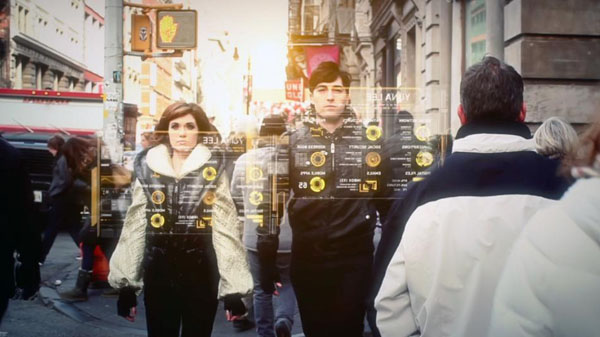
\includegraphics[width=90mm]{1.jpg}
\caption{Дополненная реальнотсь} 
\end{figure}

Всё началось с~машинного зрения. Для человека зрение настолько естественно, что большинство просто не задумывается, что кого-то, в~данном случае что-то, нужно этому учить. Хотя многие современные компьютеры выглядят совсем не глупее людей, научить их видеть "--- чрезвычайно непростая задача. Они должны не только уметь различать цвета, идентифицировать предметы, определять их границы и~классифицировать, но и~учитывать контекст, внутриклассовую изменчивость, масштаб, освещение, возможную деформацию при движении, изменении ракурса и~положения, отличать, к~примеру, отбрасываемую тень от самого предмета.
\begin{figure}[htbp]
\centering 
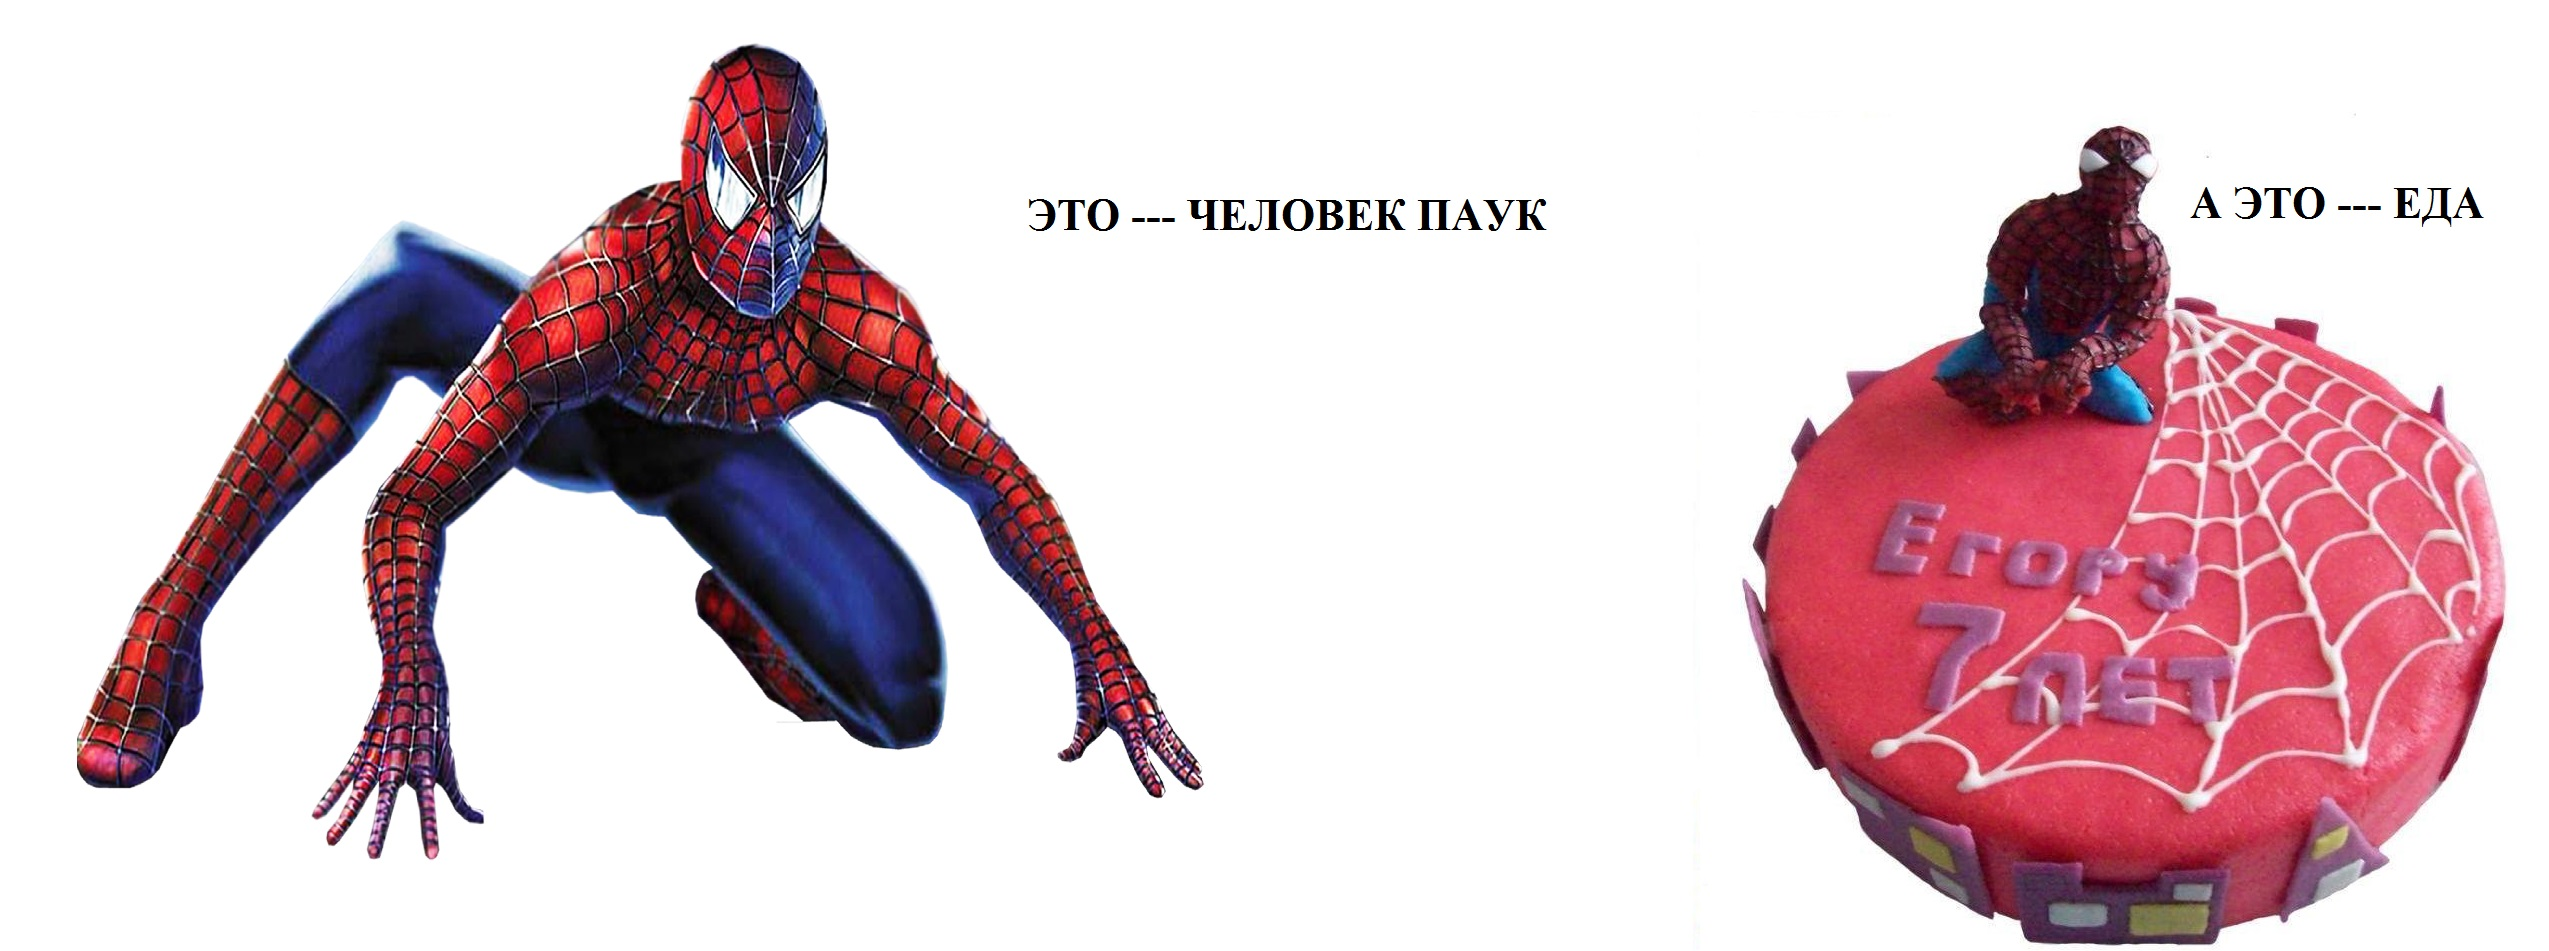
\includegraphics[width=50mm]{tt.jpg}\quad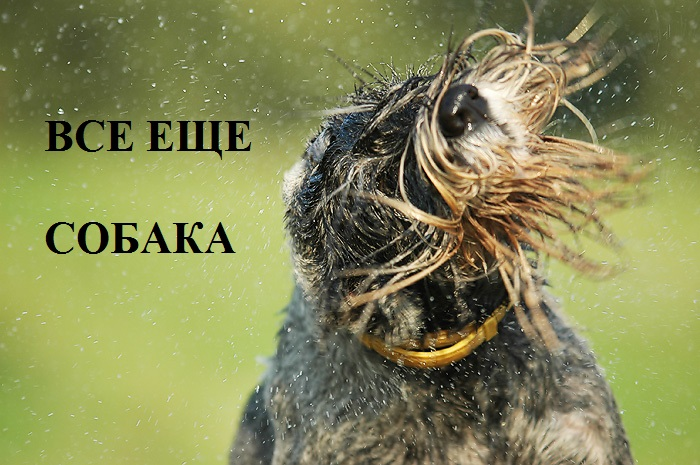
\includegraphics[width=50mm]{dd.jpg}
\caption{Заголовок 2}
\end{figure}

Однако мир не без умных людей, и~современные алгоритмы, так или иначе, позволяют решать эти проблемы. Сфера применения компьютерного зрения весьма обширна: системы моделирования объектов и~окружающей среды, медицинских изображений, рентгенов, томографий, системы видеонаблюдения и~организации информаций, а~также системы дополненной реальности и~проч. С~дополненной реальностью, несмотря на всю загадочность названия, сталкивался каждый, кто хоть раз смотрел различные спортивные мероприятия, будь то теннис, когда в~случае спорных моментов моделируется траектория полёта мяча, или футбол, где при определении офсайда возникает линия, параллельная лицевой, которая позволяет определить ближайшего к~воротам игрока.

Одна из разновидностей дополненной реальности "--- это всем известные QR-коды и~штрих коды. Несложно догадаться, где именно черпал вдохновение создатель штрих кодов, да, вы правы, в~азбуке Морзе. Однако данные линейные коды вмещают слишком мало информации, по этой причине в~1994 году в~Японии и~были изобретены двухмерные или матричные коды. Самым популярным из которых и~стал QR-код, что означает «быстрый отклик». И, если у~обычных штрихкодов объем памяти не превышал 100 байт, то у~матричных кодов данный показатель значительно выше "--- до 2048 байт (\cite{WikiDataMatrixRu}), более того информация может быть считана даже при 30\% повреждении метки! 

Что вызвало некое удивление относительно применения QR-кодов, так это использование последних на кладбищах в~Японии и~Австрии для хранения информации об~усопшем, впрочем, вернёмся к~основным техническим характеристикам. Самый маленький QR-код имеет размер $21\times21$ пиксель, в~то время как самый большой (версия 40) "--- $177\times177$ пикселей. Что касается кодировки QR-кодов, то существует 4 основных типа: цифровая (до 7089 цифр), алфавитно-цифровая (до 4296 символов), байтовая(до 2953 байт), кандзи (до 1817 иероглифов)\footnote{https://ru.wikipedia.org/wiki/QR}.

Каждому не раз приходилось сталкиваться с~QR-кодами в~жизни, некоторым даже использовали смартфоны, чтобы считать код. Но вряд ли кому-то приходило в~голову делать это вручную. А~так как в~жизни бывают разные ситуации, почему бы не восполнить данный пробел?

Для начала разберёмся, как устроен QR-код. Изначально данные, которые нужно закодировать, разбиваются на блоки в~зависимости от режима кодирования, далее прибавляется заголовок, указывающий режим и~количество блоков. Безусловно, существуют режимы с~более сложной структурой кодирования, однако из них весьма проблематично извлекать информацию вручную, поэтому остановимся на более простых случаях. После того, как записаны все информационные данные, к~ним добавляются корректирующие ошибки коды Рида-Соломона (RS), которые позволяют исправлять недочеты при чтении. Именно эти коды и~занимают большую часть QR матрицы. Перед записью в~картинку данные с~RS-кодами перемешиваются, для чего используются специальные маски. Среди имеющихся 8 алгоритмов, которые представлены на рисунке справа, выбирается наилучший, который определяется засчет системы штрафов. После этой процедуры перемешанные данные записываются на шаблонную картинку, к~которой добавляются техническая информация для декодирующих устройств\footnote{http://habrahabr.ru/post/127197/}.

Возможно, многие замечали, что QR-код можно разбить на несколько областей, у~каждой из которых индивидуальные функции, что показано на рисунке слева. Так вот, три квадрата в~углах изображения и~меньшие синхронизирующие квадратики по всему коду и~есть техническая информация для декодирующих устройств, которая позволяет нормализовать размер изображения и~его ориентацию, а~также угол, под которым сенсор расположен к~поверхности изображения. Таким образом, как вы можете догадаться, эта область абсолютно неинтересна для нас, так как не содержат никакой информации о~скрывающимся за кодом послании. Что касается полезной части кода, то ее можно разделить на две области: область, отвечающая за системную информацию, и~непосредственнно за данные. Также в~матрице содержится информация о~версии кода, от которой зависит ёмкость последнего. Так, при повышении версии добавляются специальные блоки, при высоких версиях кода не рекомендуется считывать его вручную.

Системная информация представляет собой 15~бит данных, из которых только 5~бит для нас значимы: 2~бита отвечают за уровень коррекции ошибок, а~оставшиеся~3 "--- применяемую к~данным маску. ЕщЁ 10 бит данных это BCH код, который дает возможность исправлять ошибки в~системных данных. Упомянутые ранее RS-коды, коды Рида"--~Соломона, также относятся к~классу BCH. Помимо всего прочего, для дополнительной защиты системной информации используется статическая маска, применяемая к~любой системной информации. Она имеет вид: 101010000010010. А~так как нам интересны только первые 5 бит, то маску можно сократить и~уже не так сложно запомнить: 10101. Как видно из рисунка, системная информация, отмеченная красным цветом, дублируется, что позволяет значительно понизить вероятность возникновения ошибок.

\begin{figure}
	\noindent 
	\begin{minipage}[c]{90mm} 
		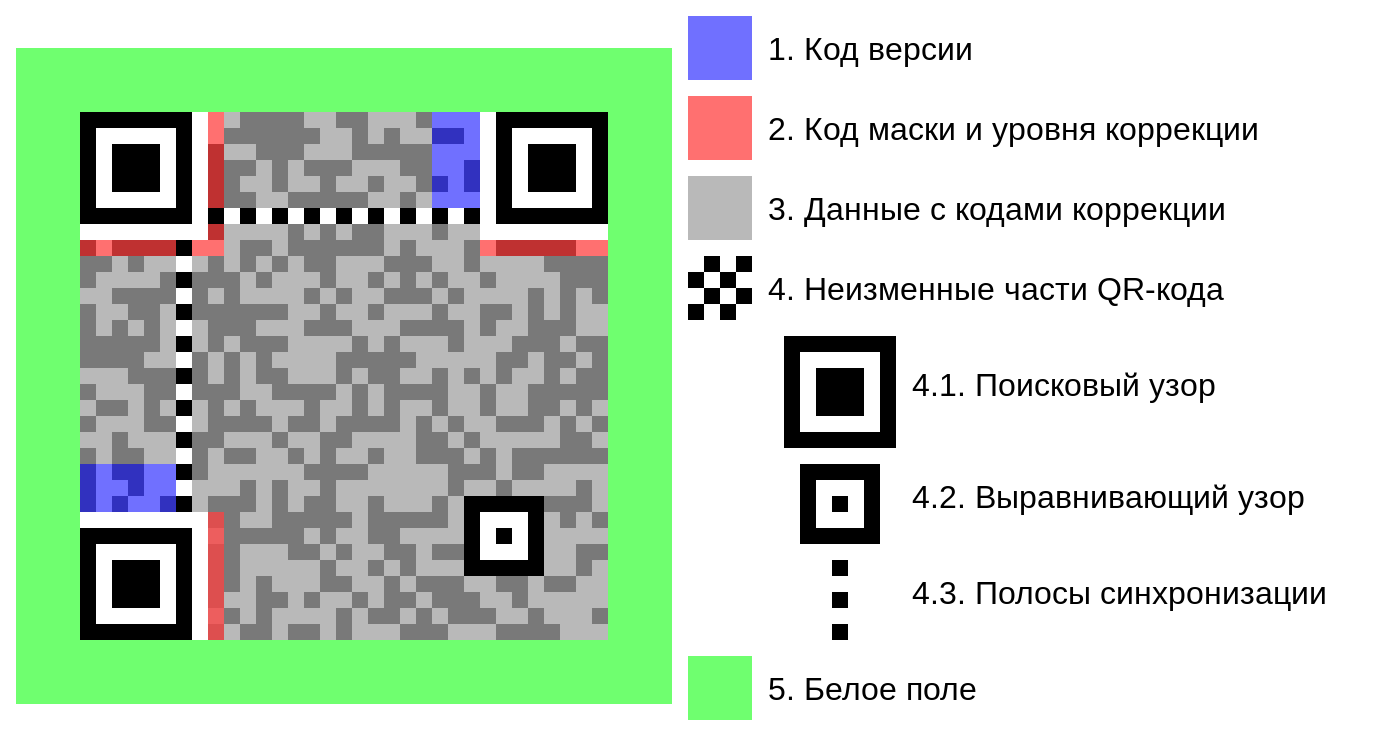
\includegraphics[width=90mm]{qr1.png} 
		\label{figLeft}
	\end{minipage}
	\hfill 
	\begin{minipage}[c]{90mm} 
		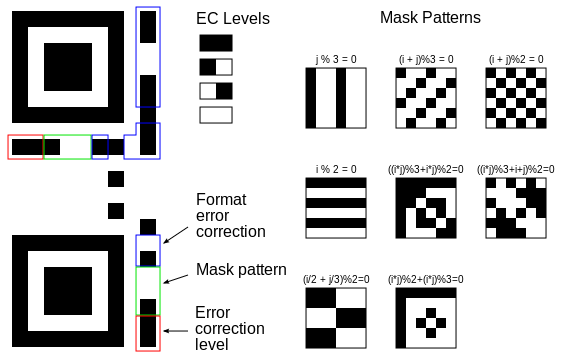
\includegraphics[width=90mm]{qr2.png}
		\label{figRight}
	\end{minipage}
\end{figure}

Таким образом, {\bf первый шаг "--- чтение первых 5 бит системной информации}.
\begin{figure}[htbp]
	\noindent
	\hfil
	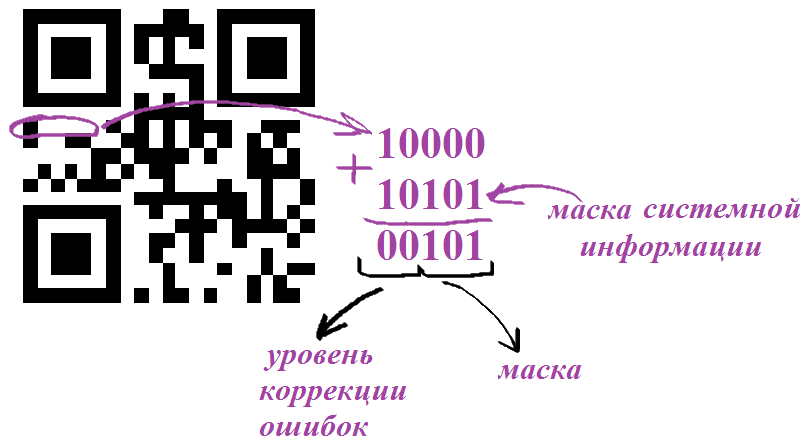
\includegraphics[width=90mm]{1.png}
	\hfil
\end{figure}

Для лучшего понимания воспользуемся кодом, сгенерированным на {\it QR Coder.ru}. Получили, что для нашего кода уровень коррекции ошибок "--- 00 "--- уровень М, позволяющий скорректировать до 15\% ошибок, маска "--- 101, соответствующая 8 картинке на рисунке (3 ряд, справа). Все возможные варианты масок и~уровней коррекции представлены в~таблице 1.

\newpage
\textbf{Шаг второй "--- определение режима кодировки.}
\begin{figure}[htbp]
	\noindent
	\hfil
	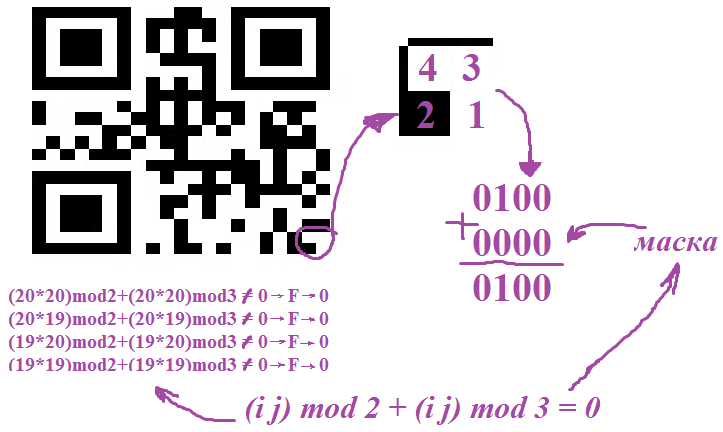
\includegraphics[width=90mm]{21.png}
	\hfil
\end{figure}

Чтобы понять с~какими данными предстоит иметь дело, необходимо изначально прочитать 4-х битный заголовок, который содержит в~себе информацию о~режиме. Заголовок находится в~правом нижнем углу матрицы, причём читать его надо змейкой, начиная справа. После извлечения 4-х бит, описывающих режим, необходимо применить к~ним маску. Маска определяется выражением, приведённым в~таблице, в~нашем случае "--- {\it (i j) mod 2 + (i j) mod 3 = 0} . Если данное выражение сводится к~{\it TRUE} для бита с~координатами (i,j), то бит инвертируется, иначе все остаётся без изменений. Начало координат в~левом верхнем углу (0,0), в~матрице $21\times21$ бит, квадрат, таким образом, бит, находящийся в~правом нижнем углу имеет координаты (20,20). Получили 0100, что соответствует 8-битному режиму.

\textbf{Шаг третий "--- теперь можно читать данные.}
\begin{figure}[htb]
	\noindent
	\hfil
	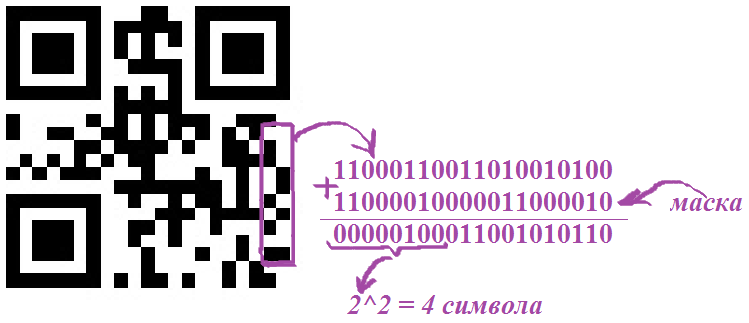
\includegraphics[width=90mm]{31.png}
	\hfil
\end{figure}

Необходимость определения режима кодирования обуславливается тем, что от него зависит длина блоков данных, которая также варьируется для различных версий кода. Для 1 - 9 версии кода: в~числовом режиме используются 10-битные или 4-х битные блоки, если в~10-битном объёме нет необходимости, в~буквенно-числовом режиме "--- 9-битные блоки, при 8-битном (байтном) режиме "--- 8-битные блоки. Причем первым блок после указателя режима "--- это количество символов. Таким образом, для определения количества символов расшифровываем следующие 8 бит кода (змейком, начиная справа) и~применяем маску. Видно, что в~коде зашифровано 4 символа, поэтому необходимо перейти к~чтению следующего столбца для извлечения всех 4-х блоков информации.

\begin{figure}[htbp]
	\noindent
	\hfil
	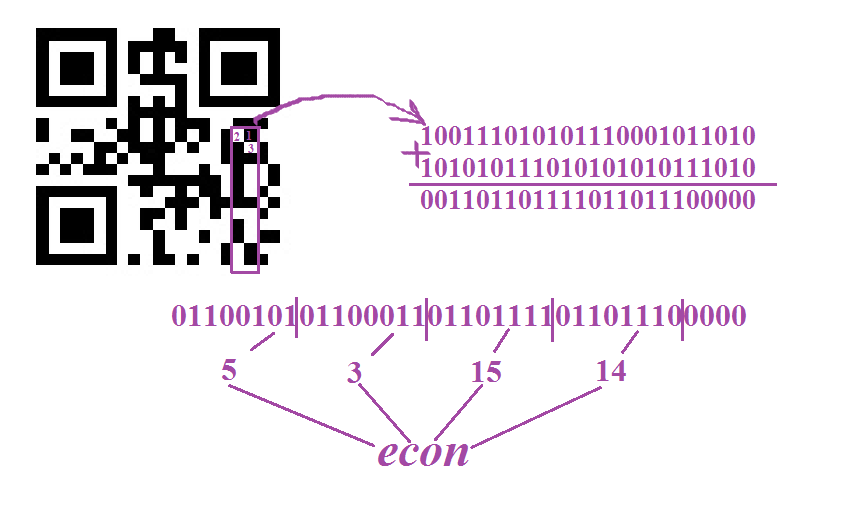
\includegraphics[width=90mm]{41.png}
	\hfil
\end{figure}

Снова считываем данные по такому же алгоритму, главное отличие "--- биты надо отсчитывать змейкой, но с~правого верхнего угла. Далее полученный набор из 0 и~1 делим на 4 блока по 8 бит в~каждом. Текст в~8-битном режиме многие онлайн генераторы QR кодируют, используя {\it ASCII}. Таким образом, первые 4 элемента блока указывают на регистр, 0110 соответствует нижнему регистру букв, 0100 "--- верхнему, вторые 4 элемента "--- это число, равное номеру буквы в~алфавите. Как можно заметить, все наши буквы "--- маленькие, далее получаем числа 5, 3, 15 и~14, и~находим нужные нам буквы. Так, в~коде была зашифрована часть слова, а~именно {\bf econ}, а~какого именно слова economics или econometrics, или что-то ещё "--- пусть каждый решает для себя сам!


\begin{table}[hbtp]
\centering
\begin{tabular}{||c|l||}
\hline 
\multicolumn{2}{|c|}{\bf Возможные маски}\\ 
\hline
{\bf 000} & (i + j) mod 2 = 0\\
{\bf 001} & i mod 2 = 0\\
{\bf 010}	& j mod 3 = 0\\
{\bf 011}	& (i + j) mod 3 = 0\\
{\bf 100}	& ((i div 2) + (j div 3)) mod 2 = 0\\
{\bf 101}	& (i j) mod 2 + (i j) mod 3 = 0\\
{\bf 110}	& ((i j) mod 2 + (i j) mod 3) mod 2 = 0\\
{\bf 111}	& ((i+j) mod 2 + (i j) mod 3) mod 2 = 0\\
\hline 
\multicolumn{2}{|c|}{\bf Возможные уровни коррекции ошибок}\\  
\hline
{\bf  01} & L\\
{\bf  00} & M\\
{\bf  11} & Q\\
{\bf  10} & H\\
\hline
\multicolumn{2}{|c|}{\bf Возможные режимы}\\  
\hline
{\bf  0111} & ECI\\
{\bf  0001} & Числовые\\
{\bf  0010} & Буквенно-числовые\\
{\bf  0100} & 8-битный (байтный)\\
{\bf  1000} & Kanji\\
{\bf  0011} & Структурированное дополнение\\
{\bf  0101} & FNC1 (1-я позиция)\\
{\bf  1001} & FNC1 (2-я позиция)\\
\hline
\end{tabular}
\caption{Заг та} \label{tab:un5} 
\end{table}

\begin{center}
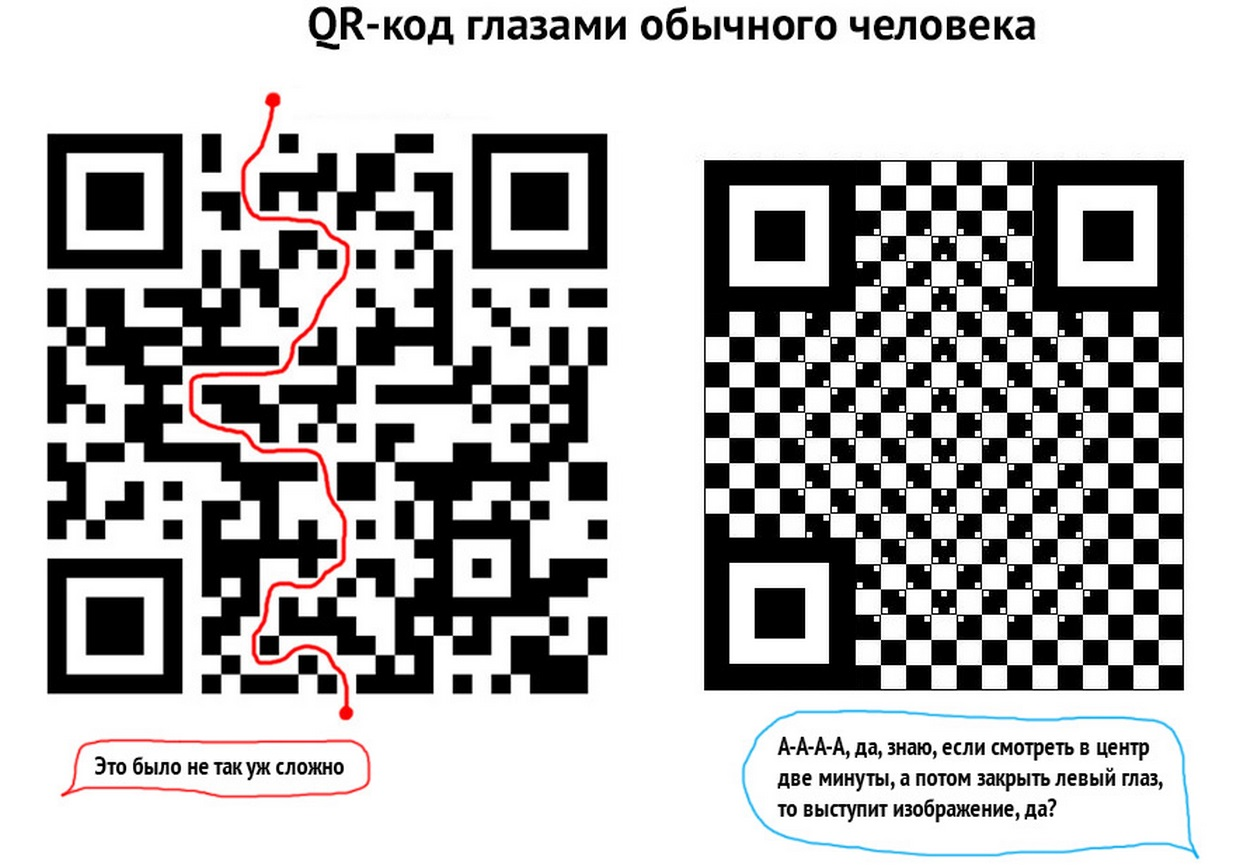
\includegraphics[width=120mm]{qr.jpg} 
\end{center}

\printbibliography

\end{document}